\documentclass[tikz,border=8pt]{standalone}
\usepackage{amsmath,amssymb}
\usetikzlibrary{arrows.meta,calc,decorations.markings,decorations.pathmorphing,patterns,shapes.geometric,positioning}

\begin{document}
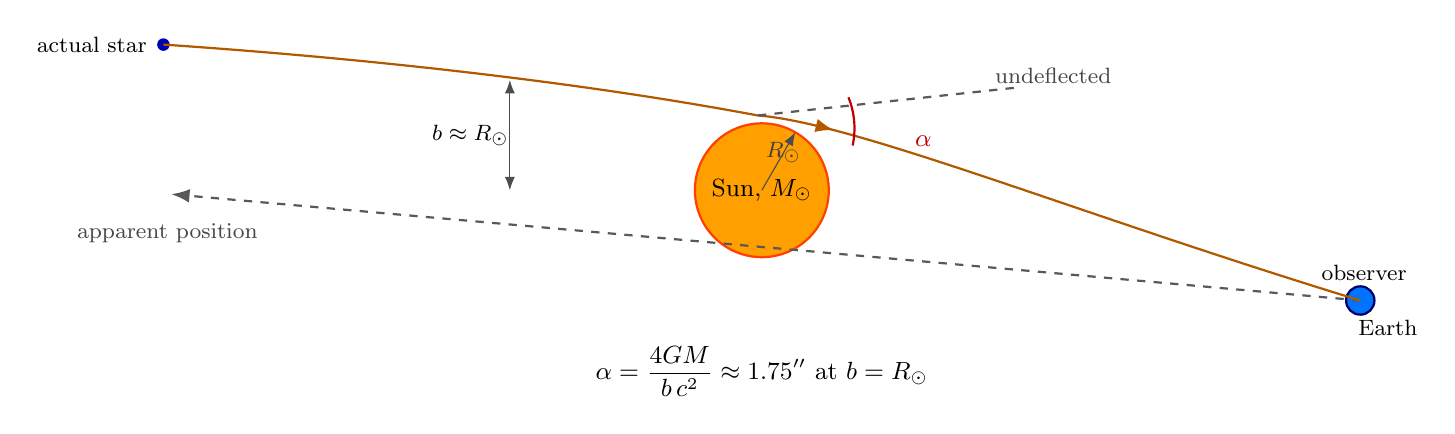
\begin{tikzpicture}[>=Latex,
    raylight/.style={thick, orange!70!black},
    apparent/.style={dashed, thick, gray!70!black},
    arc/.style={thick, red!75!black}]

  % Sun
  \fill[orange!75!yellow] (0,0) circle (0.85);
  \draw[thick, orange!50!red] (0,0) circle (0.85);
  \node[font=\small] at (0,0) {Sun, $M_\odot$};
  \draw[->, thin, gray!60!black] (0,0) -- (60:0.85);
  \node[font=\footnotesize, gray!50!black] at (60:0.55) {$R_\odot$};

  % Actual star (far left)
  \node[circle, fill=blue!70!black, inner sep=1.6pt, label={left:\footnotesize actual star}] (S) at (-7.6, 1.85) {};

  % Earth (far right)
  \fill[blue!55!cyan] (7.6, -1.4) circle (0.18);
  \draw[thick, blue!40!black] (7.6, -1.4) circle (0.18);
  \node[font=\footnotesize] at (7.95, -1.75) {Earth};
  \node[font=\footnotesize] at (7.65, -1.05) {observer};

  % Apparent position (dashed straight line from observer back through tangent of incoming ray)
  % Apparent direction is tangent to the deflected ray at observer; star appears along that tangent (extension)
  \node[font=\footnotesize, gray!55!black] at (-7.55, -0.55) {apparent position};
  \draw[apparent, ->] (7.6,-1.4) -- (-7.5, -0.05);

  % Bent light path: from star to grazing the Sun, then to Earth.
  % We approximate as two straight segments meeting near the limb of the sun on the upper side.
  \coordinate (A) at (-7.6, 1.85);
  \coordinate (G) at (-0.05, 0.95); % grazing point near top of sun
  \coordinate (E) at (7.6, -1.4);

  % Use a smooth curve for the light: Bezier through the grazing region
  \draw[raylight, postaction={decorate,
        decoration={markings, mark=at position 0.55 with {\arrow{Latex}}}}]
    (A) .. controls (-3.2, 1.55) and (-0.6, 1.05) .. (G)
        .. controls (1.2, 0.85) and (4.0, -0.30) .. (E);

  % Impact parameter b: vertical distance from sun center to incoming straight ray
  \draw[<->, thin, black!70] (-3.2, 0) -- (-3.2, 1.40);
  \node[font=\footnotesize] at (-3.7, 0.70) {$b\approx R_\odot$};

  % Deflection angle alpha at the grazing point (between incoming direction and outgoing direction)
  % Incoming direction near G is roughly along (G - A)
  % Outgoing direction near G is roughly along (E - G)
  % Show an arc and label alpha
  \draw[arc] (1.10, 1.18) arc[start angle=22, end angle=-12, radius=1.05];
  \node[font=\small, red!75!black] at (2.05, 0.62) {$\alpha$};

  % Formula
  \node[font=\small, align=center] at (0, -2.30)
    {$\alpha = \dfrac{4GM}{b\,c^{2}} \approx 1.75''$ at $b=R_\odot$};

  % Faint extension of the incoming light path showing where the star "would" appear if undeflected.
  % This visually anchors "apparent position".
  \draw[apparent] (G) -- (3.2, 1.30);
  \node[font=\footnotesize, gray!55!black] at (3.7, 1.45) {undeflected};

\end{tikzpicture}
\end{document}
